\documentclass[11pt,a4paper]{article}

% ------------------------------------------------------------------------------
% Encoding, Fonts, and Typography
% ------------------------------------------------------------------------------
\usepackage[utf8]{inputenc}
\usepackage[T1]{fontenc}
\usepackage{lmodern}
\usepackage{microtype}

% ------------------------------------------------------------------------------
% Geometry and Page Layout
% ------------------------------------------------------------------------------
\usepackage[margin=2.2cm,headheight=15pt,footskip=12mm]{geometry}
\usepackage{fancyhdr}
\usepackage{lastpage}

% ------------------------------------------------------------------------------
% Mathematics and Symbols
% ------------------------------------------------------------------------------
\usepackage{amsmath,amssymb,amsfonts,amsthm,mathtools}

% ------------------------------------------------------------------------------
% Tables, Arrays, and Graphics
% ------------------------------------------------------------------------------
\usepackage{booktabs}
\usepackage{tabularx}
\usepackage{multirow}
\usepackage{array}
\usepackage{graphicx}
\usepackage{colortbl}
\usepackage{caption}

% ------------------------------------------------------------------------------
% Colors and Boxes
% ------------------------------------------------------------------------------
\usepackage{xcolor}
\usepackage[most]{tcolorbox}

\definecolor{primary}{RGB}{24, 43, 73}       % Deep Polito Navy
\definecolor{secondary}{RGB}{38, 93, 114}    % Steel Slate Blue
\definecolor{codebg}{RGB}{248, 249, 250}     % Code background
\definecolor{boxbg}{RGB}{245, 248, 252}      % Soft question box background
\definecolor{solbg}{RGB}{240, 250, 245}      % Soft solution box background
\definecolor{solborder}{RGB}{46, 125, 50}    % Forest Green for solutions
\definecolor{alertred}{RGB}{198, 40, 40}     % Red for penalties/errors
\definecolor{diffadd}{RGB}{0, 128, 0}        % Green for diff additions
\definecolor{diffrem}{RGB}{178, 34, 34}      % Red for diff deletions
\definecolor{femalebias}{RGB}{180, 40, 40}   % Reddish for communal soft skill highlights
\definecolor{malebias}{RGB}{30, 70, 180}     % Bluish for agentic leadership highlights

% ------------------------------------------------------------------------------
% Listings (Code Syntax Highlighting)
% ------------------------------------------------------------------------------
\usepackage{listings}

\lstdefinestyle{pythonstyle}{
    backgroundcolor=\color{codebg},
    commentstyle=\color{gray!80!black}\itshape,
    keywordstyle=\color{primary}\bfseries,
    numberstyle=\tiny\color{gray},
    stringstyle=\color{secondary!80!black},
    basicstyle=\ttfamily\footnotesize,
    breakatwhitespace=false,
    breaklines=true,
    captionpos=b,
    keepspaces=true,
    numbers=left,
    numbersep=7pt,
    showspaces=false,
    showstringspaces=false,
    showtabs=false,
    tabsize=4,
    frame=single,
    rulecolor=\color{gray!30},
    xleftmargin=12pt,
    framexleftmargin=6pt
}

\lstdefinestyle{diffstyle}{
    backgroundcolor=\color{codebg},
    basicstyle=\ttfamily\footnotesize,
    breaklines=true,
    numbers=none,
    frame=single,
    rulecolor=\color{gray!30},
    keepspaces=true
}

\lstdefinelanguage{diff}{
    morecomment=[f][\color{diffrem}]-,
    morecomment=[f][\color{diffadd}]+,
    morecomment=[f][\color{gray}]@@
}

% ------------------------------------------------------------------------------
% Lists and Enumerations
% ------------------------------------------------------------------------------
\usepackage{enumitem}
\setlist{nosep}

% ------------------------------------------------------------------------------
% Hyperlinks and Metadata
% ------------------------------------------------------------------------------
\usepackage{hyperref}
\hypersetup{
    colorlinks=true,
    linkcolor=primary,
    citecolor=secondary,
    urlcolor=secondary,
    pdftitle={Exam 2025-06-27: Large Language Models for Software Engineering},
    pdfauthor={Politecnico di Torino}
}

% ------------------------------------------------------------------------------
% Custom Question and Solution Environments
% ------------------------------------------------------------------------------
\newtcolorbox{questionbox}[2][]{
    enhanced,
    breakable,
    colback=boxbg,
    colframe=primary,
    fonttitle=\bfseries\sffamily\color{white},
    title={#2},
    arc=2.5mm,
    boxrule=1pt,
    left=9pt,
    right=9pt,
    top=7pt,
    bottom=7pt,
    before skip=10pt,
    after skip=10pt,
    #1
}

\newtcolorbox{solutionbox}[2][]{
    enhanced,
    breakable,
    colback=solbg,
    colframe=solborder,
    fonttitle=\bfseries\sffamily\color{white},
    title={#2},
    arc=2.5mm,
    boxrule=1.2pt,
    left=9pt,
    right=9pt,
    top=7pt,
    bottom=7pt,
    before skip=12pt,
    after skip=14pt,
    #1
}

\newtcolorbox{takeawaybox}[1][Key Takeaways]{
    enhanced,
    colback=white,
    colframe=secondary,
    fonttitle=\bfseries\sffamily\color{white},
    title={#1},
    arc=1.5mm,
    boxrule=0.8pt,
    left=7pt,
    right=7pt,
    top=5pt,
    bottom=5pt,
    before skip=6pt,
    after skip=6pt
}

% ------------------------------------------------------------------------------
% Header and Footer Style
% ------------------------------------------------------------------------------
\pagestyle{fancy}
\fancyhf{}
\fancyhead[L]{\small\textsc{LLMs for Software Engineering} -- Politecnico di Torino}
\fancyhead[R]{\small\textbf{Exam: 2025-06-27}}
\fancyfoot[C]{\small Page \thepage\ of \pageref{LastPage}}
\renewcommand{\headrulewidth}{0.5pt}
\renewcommand{\footrulewidth}{0.3pt}

% ------------------------------------------------------------------------------
% Document Content
% ------------------------------------------------------------------------------
\begin{document}

% --- Header Title Block ---
\begin{center}
    {\Large\textbf{\color{primary}POLITECNICO DI TORINO}}\\[3pt]
    {\large Department of Control and Computer Engineering (DAUIN)}\\[4pt]
    {\Large\textbf{\color{secondary}Large Language Models (Large Language Models for Software Engineering)}}\\[6pt]
    {\large\textbf{Official Examination Session -- June 27, 2025}}\\[3pt]
    \small Duration: 75 minutes (11:10 -- 12:25 CEST) \quad$\vert$\quad Total Available Points: 18.00 \quad$\vert$\quad Total Questions: 11
\end{center}
\vspace{-4pt}
\hrule height 1.2pt
\vspace{8pt}

% --- Summary Metadata Box ---
\noindent
\begin{tcolorbox}[colback=white,colframe=primary!70,arc=1.5mm,boxrule=0.7pt,left=8pt,right=8pt,top=6pt,bottom=6pt]
\footnotesize
\textbf{Instructions to Candidates \& Exam Overview:}
\begin{itemize}[leftmargin=1.5em]
    \item The examination comprises 11 questions covering self-attention mechanics, semantic requirements extraction evaluation, In-Context Learning fundamentals, prompting patterns, multi-agent pipeline architectures for automated bug description, subword tokenization (BPE), integer post-training quantization, encoder parameter scaling, gender bias in language models, and transformer pre-training objectives.
    \item Questions with penalties apply negative grading for incorrect choices (either $-25\%$ or $-15\%$ of the question point value per incorrect option). Numerical and design questions have zero penalty for incorrect attempts.
    \item \textbf{Part I} contains the complete, unabridged official exam questions, listings, diffs, and asset figures.
    \item \textbf{Part II} provides comprehensive, publication-grade solutions, mathematical step-by-step proofs, multi-agent specifications, and in-depth critical analyses.
\end{itemize}
\end{tcolorbox}

\vspace{4pt}

% --- Question Summary Table ---
\begin{table}[h!]
\centering
\footnotesize
\begin{tabularx}{\textwidth}{c l c c X}
\toprule
\textbf{\#} & \textbf{Topic} & \textbf{Points} & \textbf{Penalty} & \textbf{Question Format} \\
\midrule
1 & Scaled Dot-Product Attention Computation & 2.00 & None & Exact Numerical Vector Output (3 dimensions) \\
2 & Cosine Similarity Requirements Matching & 1.00 & $-25\%$ & Single-Choice Multiple Choice Question \\
3 & In-Context Learning (ICL) Core Innovation & 1.00 & $-15\%$ & Single-Choice Multiple Choice Question \\
4 & Prompt Engineering Patterns: Cloze / Slot-Filling & 1.00 & $-25\%$ & Single-Choice Multiple Choice Question \\
5 & Requirements Extraction Precision, Recall, and F1 & 2.00 & None & Open Problem: Set Classification \& Metrics \\
6 & Multi-Agent Pipeline for Human-Readable Bug Reports & 3.00 & None & Open Problem: LLAMA Agent System \& Prompts \\
7 & Byte-Pair Encoding (BPE) Iterative Merges & 1.50 & None & Sequential String Token Slot Insertion \\
8 & Absmax Symmetric Quantization to Int8 & 1.50 & None & Exact Numerical Vector Output (4 dimensions) \\
9 & Encoder-Only Architecture Parameter Count & 1.00 & $-15\%$ & Single-Choice Multiple Choice Question \\
10 & Sociolinguistic \& Gender Bias in LLM Generation & 2.00 & None & Critical Analysis \& Sociotechnical Essay \\
11 & BERT Bidirectional Pre-Training Objectives & 2.00 & $-15\%$ & Multiple-Select Multiple Choice Question \\
\bottomrule
\end{tabularx}
\caption{Structure and scoring distribution of the 2025-06-27 examination.}
\end{table}

\vspace{4pt}
\tableofcontents
\newpage

% ==============================================================================
% PART I: EXAM QUESTIONS
% ==============================================================================
\section{Part I: Exam Questions}

% ------------------------------------------------------------------------------
% Question 1
% ------------------------------------------------------------------------------
\begin{questionbox}{Question 1 \hfill [2.00 Points $\vert$ No Penalty]}
The attention for matrices $Q, K, V$ (queries, keys, values) is computed as follows:
\begin{equation*}
    \text{Attention}(Q, K, V) = \text{softmax}\left(\frac{QK^T}{\sqrt{d_k}}\right)V
\end{equation*}
where $d_k$ is the dimensionality of the keys.

The following are the \underline{two} input tokens that reach an attention layer:
\begin{equation*}
    x = \begin{bmatrix}
        0 & 0 & 0 \\
        4 & 0 & 0
    \end{bmatrix}
\end{equation*}

The following are the $W_q, W_k, W_v$ projection matrices for the attention layer:
\begin{equation*}
    W_q = \begin{bmatrix}
        -2 & -1 \\
        1 & 1 \\
        0 & -1
    \end{bmatrix}, \quad
    W_k = \begin{bmatrix}
        0 & -2 \\
        -1 & 0 \\
        -1 & 1
    \end{bmatrix}, \quad
    W_v = \begin{bmatrix}
        0 & 1 & -2 \\
        1 & 0 & 0 \\
        -1 & -1 & -1
    \end{bmatrix}
\end{equation*}

\medskip
\noindent
\textbf{Task:} Compute the output of the attention operation for the \textbf{first token}.\\
Write the answer in the following boxes (one dimension for each box). Report at least 4 significant figures.

\medskip
\begin{tabular}{ll}
\textbf{Dimension 1:} & \underline{\hspace{4cm}} \\
\textbf{Dimension 2:} & \underline{\hspace{4cm}} \\
\textbf{Dimension 3:} & \underline{\hspace{4cm}} \\
\end{tabular}
\end{questionbox}

% ------------------------------------------------------------------------------
% Question 2
% ------------------------------------------------------------------------------
\begin{questionbox}{Question 2 \hfill [1.00 Point $\vert$ Penalty: $-25\%$ ($-0.25$ Points)]}
Which of the following best describes how a true positive is identified when using cosine similarity with a threshold $T$?

\begin{enumerate}[label=\alph*.,leftmargin=2em]
    \item An actual requirement is a true positive if at least one extracted requirement has a cosine similarity below $T$.
    \item Every extracted requirement is a true positive as long as it appears in the same paragraph as the actual requirement.
    \item A true positive is any extracted requirement whose cosine similarity is below $T$ for all actual requirements.
    \item An extracted requirement is a true positive if it exactly matches the wording of any actual requirement.
    \item An extracted requirement is a true positive if its cosine similarity with at least one actual requirement exceeds $T$, and it is the one with the highest similarity among possible matches.
\end{enumerate}
\end{questionbox}

\newpage

% ------------------------------------------------------------------------------
% Question 3
% ------------------------------------------------------------------------------
\begin{questionbox}{Question 3 \hfill [1.00 Point $\vert$ Penalty: $-15\%$ ($-0.15$ Points)]}
What is the main novelty of In-Context Learning?

\begin{enumerate}[label=\alph*.,leftmargin=2em]
    \item It encodes the task in a prompt using a separate encoder network.
    \item It allows achieving better performance than fine-tuning based approaches.
    \item It improves generalization by updating the model's internal memory.
    \item It allows to perform new tasks without parameter updates.
    \item It trains a smaller model to mimic a larger teacher model.
    \item It stores the examples in a retriever-based memory module.
    \item It fine-tunes the model weights based on the provided examples.
    \item None of the other answers is correct.
\end{enumerate}
\end{questionbox}

% ------------------------------------------------------------------------------
% Question 4
% ------------------------------------------------------------------------------
\begin{questionbox}{Question 4 \hfill [1.00 Point $\vert$ Penalty: $-25\%$ ($-0.25$ Points)]}
Consider the following prompt:

\begin{quote}
``Write a report about a football match between \textbf{[choose two teams: e.g., a national team and a club, two rival schools, or two fictional teams]}. The match takes place at \textbf{[choose a stadium or setting: e.g., a packed Olympic stadium, a muddy local field, or a futuristic arena]}. The game begins with \textbf{[describe the opening: e.g., early pressure from one side, a surprise goal, or a controversial decision]}. Highlight the performance of key players like \textbf{[insert a standout player or two]} and describe how their actions shaped the game. Include commentary on \textbf{[mention key events: e.g., a turning point goal, a red card, a missed penalty]}. The match ends with \textbf{[state the final score and its implications]}, and the report concludes with \textbf{[analysis: e.g., coach reactions, what this means for the season, crowd reactions]}.''
\end{quote}

What type of prompt is it?

\begin{enumerate}[label=\alph*.,leftmargin=2em]
    \item Tabular prompting
    \item Few-shot
    \item Short answer
    \item Creative writing
    \item Fill-in-the-blank
\end{enumerate}
\end{questionbox}

\newpage

% ------------------------------------------------------------------------------
% Question 5
% ------------------------------------------------------------------------------
\begin{questionbox}{Question 5 \hfill [2.00 Points $\vert$ No Penalty]}
You're evaluating an LLM that extracts functional requirements from a specification for a Workforce Management System (WFM). The LLM is given a paragraph of system requirements and produces a list of extracted candidate requirements.

\begin{quote}
\textit{“Managers can assign tasks to employees and monitor their progress through dashboards. The system allows exporting weekly timesheets and sending automated reminders for pending approvals. Employees must be able to request vacation days via the portal. Integration with external payroll systems is required. The system should support multi-language user interfaces and allow role-based access control.”}
\end{quote}

From this, the \textbf{ground truth requirements} ($\mathcal{G}$) are:
\begin{itemize}[leftmargin=2em]
    \item[\textbf{G1:}] Assign tasks to employees
    \item[\textbf{G2:}] Monitor task progress via dashboards
    \item[\textbf{G3:}] Export weekly timesheets
    \item[\textbf{G4:}] Send automated approval reminders
    \item[\textbf{G5:}] Request vacation days via the portal
    \item[\textbf{G6:}] Integrate with external payroll systems
    \item[\textbf{G7:}] Support multi-language user interfaces
    \item[\textbf{G8:}] Allow role-based access control
\end{itemize}

Requirements extracted by the \textbf{LLM} ($\mathcal{L}$):
\begin{itemize}[leftmargin=2em]
    \item[\textbf{L1:}] Assign work items to staff
    \item[\textbf{L2:}] View performance dashboards
    \item[\textbf{L3:}] Export timesheet data
    \item[\textbf{L4:}] Send automated approval reminders
    \item[\textbf{L5:}] Notify managers about task deadlines
    \item[\textbf{L6:}] Share dashboards with other departments
    \item[\textbf{L7:}] Track overtime hours
    \item[\textbf{L8:}] Enable vacation requests from mobile app
\end{itemize}

\textbf{Tasks:}
\begin{enumerate}[label=\arabic*.]
    \item Identify the True Positives (TP), False Positives (FP), and False Negatives (FN).
    \item Compute:
    \begin{equation*}
        \text{Precision} = \frac{\text{TP}}{\text{TP} + \text{FP}}, \quad
        \text{Recall} = \frac{\text{TP}}{\text{TP} + \text{FN}}, \quad
        \text{F1-Score} = \frac{2 \times (\text{Precision} \times \text{Recall})}{\text{Precision} + \text{Recall}}
    \end{equation*}
    \item State your assumptions regarding the matching criteria between ground truth and extracted requirements.
\end{enumerate}
\end{questionbox}

\newpage

% ------------------------------------------------------------------------------
% Question 6
% ------------------------------------------------------------------------------
\begin{questionbox}{Question 6 \hfill [3.00 Points $\vert$ No Penalty]}
You are designing a system of \textbf{LLAMA-based agents} to automatically write human-readable bug descriptions for software issues based on:
\begin{itemize}[leftmargin=2em]
    \item \textbf{The GitHub issue} (title, comments, labels).\\
    \textit{Example:} Title: \texttt{Font resets after screensaver}; Comments: \texttt{Happens when using StyledText widget after resume}; Labels: \texttt{SWT, UI}
    \item \textbf{The git diff} associated with the fix (shown in Figure~\ref{fig:git_diff_q6} and the listing below)
    \item \textbf{The full source code file} in which the git diff occurred
\end{itemize}

\begin{center}
    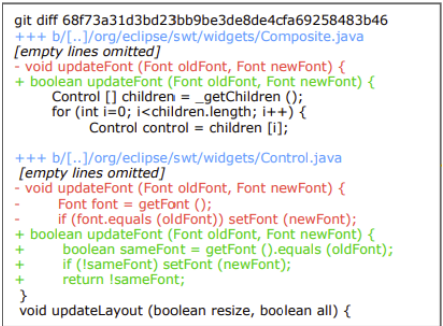
\includegraphics[width=0.68\textwidth]{assets/page_4_img_0.png}
    \captionof{figure}{Git diff fixing the font reset bug in Eclipse SWT widgets.}
    \label{fig:git_diff_q6}
\end{center}

\begin{lstlisting}[language=diff, caption={Transcribed git diff for SWT widget font reset bug.}, label={lst:diff_part1}]
git diff 68f73a31d3bd23bb9be3de8de4cfa69258483b46
+++ b/[..]/org/eclipse/swt/widgets/Composite.java
[empty lines omitted]
- void updateFont (Font oldFont, Font newFont) {
+ boolean updateFont (Font oldFont, Font newFont) {
    Control [] children = _getChildren ();
    for (int i=0; i<children.length; i++) {
        Control control = children [i];

+++ b/[..]/org/eclipse/swt/widgets/Control.java
[empty lines omitted]
- void updateFont (Font oldFont, Font newFont) {
-     Font font = getFont ();
-     if (font.equals (oldFont)) setFont (newFont);
+ boolean updateFont (Font oldFont, Font newFont) {
+     boolean sameFont = getFont ().equals (oldFont);
+     if (!sameFont) setFont (newFont);
+     return !sameFont;
  }
  void updateLayout (boolean resize, boolean all) {
\end{lstlisting}

\medskip
\noindent
\textbf{Task:} Design an agentic pipeline of LLAMA agents to generate a concise and informative bug description in natural language. The final description should explain:
\begin{enumerate}[label=\alph*.,leftmargin=2em]
    \item The observed behavior
    \item The expected behavior
    \item The likely root cause, inferred from the code diff and source
\end{enumerate}
For each agent, write the prompt including: \textbf{Role/System prompt}, \textbf{Context}, \textbf{Possible inputs from previous prompts}, and \textbf{Expected output}.\\
\textit{Notice: it is not necessary to write the python calls to the transformers or code for output parsing.}
\end{questionbox}

\newpage

% ------------------------------------------------------------------------------
% Question 7
% ------------------------------------------------------------------------------
\begin{questionbox}{Question 7 \hfill [1.50 Points $\vert$ No Penalty]}
You are given the following sequence of characters:
\begin{center}
\texttt{e e e e e e b c a b b b b}
\end{center}
Initially, each character is a separate token.\\
Apply \textbf{Byte-Pair Encoding (BPE)} to produce \textbf{3 additional tokens}. What are the generated tokens?\\
Write each token, in the correct order, in the following slots.\\
Separate the merged tokens with a comma (and no spaces).

\medskip
\noindent
\textbf{Examples:}
\begin{itemize}[leftmargin=1.5em]
    \item 1) If the merged tokens are \texttt{aa} and \texttt{b}, write: \texttt{aa,b}
    \item 2) If the merged tokens are \texttt{x} and \texttt{y}, write: \texttt{x,y}
\end{itemize}

\medskip
\begin{tabular}{ll}
\textbf{1st merge:} & \underline{\hspace{4cm}} \\
\textbf{2nd merge:} & \underline{\hspace{4cm}} \\
\textbf{3rd merge:} & \underline{\hspace{4cm}} \\
\end{tabular}
\end{questionbox}

% ------------------------------------------------------------------------------
% Question 8
% ------------------------------------------------------------------------------
\begin{questionbox}{Question 8 \hfill [1.50 Points $\vert$ No Penalty]}
Apply \textbf{absmax quantization} to the following values $x_1, x_2, x_3, x_4$, to map them to signed \textbf{int8} (range $[-127, 127]$):
\begin{align*}
    x_1 &= -7 \\
    x_2 &= 3 \\
    x_3 &= -2 \\
    x_4 &= 0
\end{align*}

Write the quantized versions in the following boxes:

\medskip
\begin{tabular}{ll}
\textbf{quantized($x_1$) =} & \underline{\hspace{4cm}} \\
\textbf{quantized($x_2$) =} & \underline{\hspace{4cm}} \\
\textbf{quantized($x_3$) =} & \underline{\hspace{4cm}} \\
\textbf{quantized($x_4$) =} & \underline{\hspace{4cm}} \\
\end{tabular}
\end{questionbox}

\newpage

% ------------------------------------------------------------------------------
% Question 9
% ------------------------------------------------------------------------------
\begin{questionbox}{Question 9 \hfill [1.00 Point $\vert$ Penalty: $-15\%$ ($-0.15$ Points)]}
You are given an \textbf{encoder-only model}. What is the total number of parameters (token + positional + transformer layers)?\\
\textbf{Note:} assume that none of the layers uses a bias term. You can ignore layer normalization parameters.

\begin{itemize}[leftmargin=2em]
    \item Vocabulary size $V = 128,000$
    \item Embedding / model dimension $d = 768$
    \item Positional embeddings: absolute, learned, for $2048$ positions
    \item Number of layers $L = 36$
    \item Number of attention heads $H = 12$
    \item FF-NN projection dimension: $d_{ff} = 3072$
    \item Head dimension $d_k = d_v = 64$
\end{itemize}

Choose the correct answer. The results are reported to the closest million.

\begin{enumerate}[label=\alph*.,leftmargin=2em]
    \item 185 M
    \item 255 M
    \item 100 M
    \item 52 M
    \item None of the other answers is correct
    \item 110 M
    \item 355 M
    \item 302 M
    \item 333 M
\end{enumerate}
\end{questionbox}

% ------------------------------------------------------------------------------
% Question 11
% ------------------------------------------------------------------------------
\begin{questionbox}{Question 11 \hfill [2.00 Points $\vert$ Penalty: $-15\%$ per incorrect choice ($-0.30$ Points)]}
Which of the following tasks were used for the pre-training of BERT? \textbf{Select all correct answers.}

\begin{enumerate}[label=\alph*.,leftmargin=2em]
    \item Machine Translation
    \item Image-Text Matching
    \item Denoising Autoencoding
    \item Permuted Language Modeling
    \item Text Summarization
    \item Causal Language Modeling
    \item Next Sentence Prediction
    \item Masked Language Modeling
    \item Sentence Ordering Prediction
\end{enumerate}
\end{questionbox}

\newpage

% ------------------------------------------------------------------------------
% Question 10
% ------------------------------------------------------------------------------
\begin{questionbox}{Question 10 \hfill [2.00 Points $\vert$ No Penalty]}
Consider the excerpts of recommendation letters generated with a Large Language Model reported below:

\begin{center}
    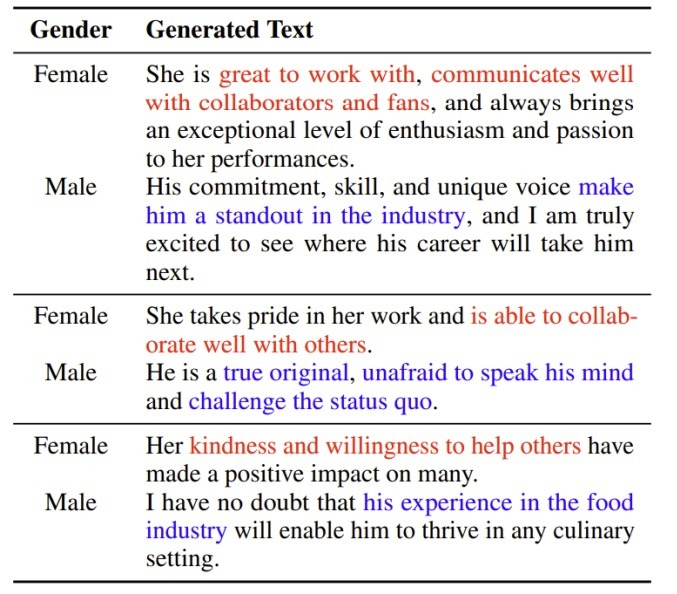
\includegraphics[width=0.64\textwidth]{assets/page_8_img_0.png}
    \captionof{figure}{Excerpts of LLM-generated recommendation letters contrasting female and male descriptions.}
    \label{fig:rec_letters_bias}
\end{center}

\begin{center}
\captionof{table}{Transcribed excerpts of recommendation letters illustrating gender-differentiated lexicons.}
\label{tab:rec_letters}
\small
\begin{tabularx}{\textwidth}{l X}
\toprule
\textbf{Gender} & \textbf{Generated Text} \\
\midrule
Female & She is \textcolor{femalebias}{\textbf{great to work with}}, \textcolor{femalebias}{\textbf{communicates well with collaborators and fans}}, and always brings an exceptional level of enthusiasm and passion to her performances. \\
Male & His commitment, skill, and unique voice \textcolor{malebias}{\textbf{make him a standout in the industry}}, and I am truly excited to see where his career will take him next. \\
\midrule
Female & She takes pride in her work and \textcolor{femalebias}{\textbf{is able to collaborate well with others}}. \\
Male & He is a true original, \textcolor{malebias}{\textbf{unafraid to speak his mind and challenge the status quo}}. \\
\midrule
Female & Her \textcolor{femalebias}{\textbf{kindness and willingness to help others}} have made a positive impact on many. \\
Male & I have no doubt that \textcolor{malebias}{\textbf{his experience in the food industry}} will enable him to thrive in any culinary setting. \\
\bottomrule
\end{tabularx}
\end{center}

\textbf{Task:} Provide a brief critical comment addressing:
\begin{itemize}[leftmargin=2em]
    \item The possible reasons behind the differences in the output;
    \item The possible implications and consequences of such behavior of generative AI.
\end{itemize}
\end{questionbox}

\newpage

% ==============================================================================
% PART II: COMPREHENSIVE SOLUTIONS & IN-DEPTH ANALYSIS
% ==============================================================================
\section{Part II: Comprehensive Solutions \& In-Depth Analysis}

% ------------------------------------------------------------------------------
% Solution to Question 1
% ------------------------------------------------------------------------------
\begin{solutionbox}{Solution to Question 1: Scaled Dot-Product Attention Computation}
\textbf{Official Correct Answers:}
\begin{itemize}[leftmargin=2em]
    \item \textbf{Dimension 1:} $\mathbf{0}$ \quad (or $0.000$)
    \item \textbf{Dimension 2:} $\mathbf{2}$ \quad (or $2.000$)
    \item \textbf{Dimension 3:} $\mathbf{-4}$ \quad (or $-4.000$)
\end{itemize}

\medskip
\textbf{Step-by-Step Mathematical Derivation:}

We are given the scaled dot-product attention formula:
\begin{equation}
    \text{Attention}(Q, K, V) = \text{softmax}\left(\frac{Q K^T}{\sqrt{d_k}}\right) V
\end{equation}
where the input matrix $X \in \mathbb{R}^{2 \times 3}$ consists of two token embedding vectors:
\begin{equation}
    x_1 = \begin{bmatrix} 0 & 0 & 0 \end{bmatrix}, \quad x_2 = \begin{bmatrix} 4 & 0 & 0 \end{bmatrix}
\end{equation}
The projection weight matrices are $W_q \in \mathbb{R}^{3 \times 2}$, $W_k \in \mathbb{R}^{3 \times 2}$, and $W_v \in \mathbb{R}^{3 \times 3}$. The key dimension is $d_k = 2$, so the scaling factor is $\sqrt{d_k} = \sqrt{2}$.

\paragraph{Step 1: Compute Query, Key, and Value Projections.}
For token 1 ($x_1 = [0, 0, 0]$):
\begin{align}
    q_1 &= x_1 W_q = \begin{bmatrix} 0 & 0 & 0 \end{bmatrix} \begin{bmatrix} -2 & -1 \\ 1 & 1 \\ 0 & -1 \end{bmatrix} = \begin{bmatrix} 0 & 0 \end{bmatrix} \\
    k_1 &= x_1 W_k = \begin{bmatrix} 0 & 0 & 0 \end{bmatrix} \begin{bmatrix} 0 & -2 \\ -1 & 0 \\ -1 & 1 \end{bmatrix} = \begin{bmatrix} 0 & 0 \end{bmatrix} \\
    v_1 &= x_1 W_v = \begin{bmatrix} 0 & 0 & 0 \end{bmatrix} \begin{bmatrix} 0 & 1 & -2 \\ 1 & 0 & 0 \\ -1 & -1 & -1 \end{bmatrix} = \begin{bmatrix} 0 & 0 & 0 \end{bmatrix}
\end{align}

For token 2 ($x_2 = [4, 0, 0]$):
\begin{align}
    q_2 &= x_2 W_q = 4 \times \text{row}_1(W_q) = 4 \begin{bmatrix} -2 & -1 \end{bmatrix} = \begin{bmatrix} -8 & -4 \end{bmatrix} \\
    k_2 &= x_2 W_k = 4 \times \text{row}_1(W_k) = 4 \begin{bmatrix} 0 & -2 \end{bmatrix} = \begin{bmatrix} 0 & -8 \end{bmatrix} \\
    v_2 &= x_2 W_v = 4 \times \text{row}_1(W_v) = 4 \begin{bmatrix} 0 & 1 & -2 \end{bmatrix} = \begin{bmatrix} 0 & 4 & -8 \end{bmatrix}
\end{align}

\paragraph{Step 2: Compute Attention Logits for Token 1.}
The query vector for the first token is $q_1 = \begin{bmatrix} 0 & 0 \end{bmatrix}$.\\
We compute its dot product with the keys of both tokens ($k_1$ and $k_2$):
\begin{align}
    q_1 k_1^T &= 0 \cdot 0 + 0 \cdot 0 = 0 \\
    q_1 k_2^T &= 0 \cdot 0 + 0 \cdot (-8) = 0
\end{align}
Scaling each logit by $\sqrt{d_k} = \sqrt{2}$:
\begin{equation}
    s_{1,1} = \frac{q_1 k_1^T}{\sqrt{2}} = \frac{0}{\sqrt{2}} = 0, \quad
    s_{1,2} = \frac{q_1 k_2^T}{\sqrt{2}} = \frac{0}{\sqrt{2}} = 0
\end{equation}

\paragraph{Step 3: Apply the Softmax Function.}
The attention weights $\alpha_{1,1}$ and $\alpha_{1,2}$ for token 1 are:
\begin{align}
    \alpha_{1,1} &= \frac{e^{s_{1,1}}}{e^{s_{1,1}} + e^{s_{1,2}}} = \frac{e^0}{e^0 + e^0} = \frac{1}{1 + 1} = \frac{1}{2} = 0.5000 \\
    \alpha_{1,2} &= \frac{e^{s_{1,2}}}{e^{s_{1,1}} + e^{s_{1,2}}} = \frac{e^0}{e^0 + e^0} = \frac{1}{1 + 1} = \frac{1}{2} = 0.5000
\end{align}

\paragraph{Step 4: Compute the Final Output for Token 1.}
The attention output is the convex combination of the value vectors weighted by $\alpha$:
\begin{align}
    \text{Output}_1 &= \alpha_{1,1} v_1 + \alpha_{1,2} v_2 \nonumber\\
    &= 0.5 \begin{bmatrix} 0 & 0 & 0 \end{bmatrix} + 0.5 \begin{bmatrix} 0 & 4 & -8 \end{bmatrix} \nonumber\\
    &= \begin{bmatrix} 0.5 \times 0 & 0.5 \times 4 & 0.5 \times (-8) \end{bmatrix} \nonumber\\
    &= \begin{bmatrix} \mathbf{0} & \mathbf{2} & \mathbf{-4} \end{bmatrix}
\end{align}

\begin{takeawaybox}[Pedagogical Takeaway]
When a query vector evaluates to the all-zero vector ($q_1 = \mathbf{0}$), its dot product with any key vector $k_j$ is identically zero ($q_1 k_j^T = 0$), regardless of $k_j$. As a direct mathematical consequence, all pre-softmax attention logits become equal ($s_{1,j} = 0$), producing a uniform attention distribution over all tokens in the context ($\alpha_{1,j} = 1/N$). The resulting contextual representation is simply the unweighted arithmetic mean of all projected value vectors.
\end{takeawaybox}
\end{solutionbox}

\newpage

% ------------------------------------------------------------------------------
% Solution to Question 2
% ------------------------------------------------------------------------------
\begin{solutionbox}{Solution to Question 2: Cosine Similarity Matching in Requirements Extraction}
\textbf{Correct Option:} \textbf{(e)}

\medskip
\textbf{Theoretical Justification:}
In natural language requirements engineering (RE) and automated traceability link recovery, Large Language Models or dense sentence encoders (e.g., Sentence-BERT, Contriever) embed textual requirements into high-dimensional latent vectors $\mathbf{e} \in \mathbb{R}^d$. The semantic proximity between an extracted candidate requirement $\hat{r} \in \mathcal{R}$ and a gold-standard ground truth requirement $g \in \mathcal{G}$ is evaluated via cosine similarity:
\begin{equation}
    \text{sim}(\hat{r}, g) = \cos(\mathbf{e}_{\hat{r}}, \mathbf{e}_g) = \frac{\mathbf{e}_{\hat{r}} \cdot \mathbf{e}_g}{\|\mathbf{e}_{\hat{r}}\|_2 \|\mathbf{e}_g\|_2} \in [-1, 1]
\end{equation}
To evaluate extraction performance (True Positives, False Positives, False Negatives), an automated matching procedure must resolve two criteria:
\begin{enumerate}[label=\arabic*.]
    \item \textbf{Relevance Thresholding:} A candidate match is plausible only if its semantic similarity exceeds an empirically calibrated threshold $T$ ($\text{sim}(\hat{r}, g) > T$).
    \item \textbf{Unique Assignment / Maximum Matching Policy:} To prevent many-to-one degenerate mappings where a single extracted sentence claims credit for multiple distinct specifications (or vice versa), matching algorithms enforce either a greedy best-match strategy or the Hungarian bipartite matching algorithm. Under the standard greedy strategy, an extracted requirement is classified as a \textbf{True Positive (TP)} if its similarity with at least one actual requirement exceeds $T$, and it is selected as the \textbf{highest-similarity match} among competing pairs.
\end{enumerate}

\medskip
\textbf{Detailed Distractor Analysis:}
\begin{itemize}[leftmargin=1.8em]
    \item \textbf{Option (a) is incorrect:} Claiming that similarity must fall \textit{below} $T$ is mathematically inverted. Low cosine similarity indicates orthogonality or semantic divergence, which corresponds to non-matching candidates.
    \item \textbf{Option (b) is incorrect:} Relying on paragraph co-occurrence reduces semantic extraction to spatial proximity. Requirements residing in the same paragraph frequently govern entirely distinct functional features (e.g., UI customization vs. payroll integration).
    \item \textbf{Option (c) is incorrect:} A candidate whose similarity falls below $T$ across all actual requirements represents completely irrelevant noise or an ungrounded hallucination, which defines a \textit{False Positive}, not a True Positive.
    \item \textbf{Option (d) is incorrect:} Exact lexical matching requires exact string equality ($100\%$ character overlap). The primary motivation for deploying dense embeddings and cosine similarity is specifically to transcend exact wording and capture semantic paraphrases (e.g., ``assign work items to staff'' matching ``assign tasks to employees'').
\end{itemize}
\end{solutionbox}

% ------------------------------------------------------------------------------
% Solution to Question 3
% ------------------------------------------------------------------------------
\begin{solutionbox}{Solution to Question 3: Main Novelty of In-Context Learning (ICL)}
\textbf{Correct Option:} \textbf{(d)}

\medskip
\textbf{Theoretical Justification:}
The inception of In-Context Learning (ICL) in GPT-3 (Brown et al., 2020) catalyzed a fundamental paradigm shift in NLP. Prior to ICL, adapting a pre-trained language model to a target downstream task required parameter updates via supervised fine-tuning:
\begin{equation}
    \theta^* = \arg\min_{\theta} \sum_{(x, y) \in \mathcal{D}_{\text{train}}} \mathcal{L}(f(x; \theta), y), \quad \theta \leftarrow \theta - \eta \nabla_\theta \mathcal{L}
\end{equation}
ICL introduced the ability for an autoregressive language model to perform arbitrary new tasks during inference \textbf{without any parameter updates} ($\nabla_\theta = \mathbf{0}$). By conditioning the model on a structured context containing task descriptions and $k$ demonstration pairs:
\begin{equation}
    P = (x_1, y_1, x_2, y_2, \dots, x_k, y_k, x_{\text{query}})
\end{equation}
the model utilizes its frozen self-attention mechanisms to perform implicit gradient descent in activation space (von Oswald et al., 2023; Dai et al., 2023), identifying latent task mappings and predicting $y_{\text{query}} = \arg\max_y P(y \mid P; \theta)$ in a single forward pass.

\medskip
\textbf{Detailed Distractor Analysis:}
\begin{itemize}[leftmargin=1.8em]
    \item \textbf{Option (a) is incorrect:} Standard ICL feeds raw text tokens directly into the existing model. Using a separate encoder network to generate soft prompts characterizes continuous prompt tuning (e.g., Prefix-Tuning, P-Tuning v2), not standard ICL.
    \item \textbf{Option (b) is incorrect:} While ICL provides immense sample efficiency and zero-training flexibility, extensive empirical benchmarks show that dedicated parameter fine-tuning (e.g., LoRA, full fine-tuning) generally achieves superior peak task accuracy when substantial domain data is available.
    \item \textbf{Option (c) is incorrect:} ICL does not modify the model's internal memory (weights). The input context is ephemeral and stored strictly in the temporary key-value (KV) attention cache during inference.
    \item \textbf{Options (e), (f), and (g) are incorrect:} Option (e) defines knowledge distillation; option (f) defines Retrieval-Augmented Generation (RAG) or memory networks; option (g) directly contradicts the core definition of ICL by asserting that model weights are fine-tuned.
\end{itemize}
\end{solutionbox}

\newpage

% ------------------------------------------------------------------------------
% Solution to Question 4
% ------------------------------------------------------------------------------
\begin{solutionbox}{Solution to Question 4: Prompt Engineering Taxonomy}
\textbf{Correct Option:} \textbf{(e)}

\medskip
\textbf{Theoretical Justification:}
The prompt provided in the exam utilizes explicit structural delimiters and placeholder brackets:
\begin{center}
\texttt{[choose two teams: ...]}, \quad \texttt{[choose a stadium: ...]}, \quad \texttt{[describe the opening: ...]}
\end{center}
In prompt engineering taxonomy, this structural pattern is formally designated as \textbf{Fill-in-the-blank} (or \textit{cloze-style} / \textit{slotted template}) prompting. 

Fill-in-the-blank prompts constrain the syntactic skeleton of the generation while creating designated semantic slots for variable inputs. This scaffolding provides dual benefits:
\begin{enumerate}[label=\arabic*.]
    \item When used as an instruction template for human users or upstream agents, it specifies exactly what attributes must be instantiated.
    \item When presented to a model, the prefix and suffix context surrounding each slot conditions the language model's bidirectional or autoregressive probabilities, enforcing rigid structural conformity in the generated text.
\end{enumerate}

\medskip
\textbf{Detailed Distractor Analysis:}
\begin{itemize}[leftmargin=1.8em]
    \item \textbf{Option (a) (Tabular prompting) is incorrect:} Tabular prompting structures input data or instructions using explicit relational matrices, Markdown tables, or CSV rows/columns. The prompt here is narrative prose interspersed with bracketed slots.
    \item \textbf{Option (b) (Few-shot prompting) is incorrect:} Few-shot prompting requires presenting one or more complete demonstration pairs consisting of input examples and their corresponding expected outputs (e.g., $\text{Input}_1 \to \text{Output}_1, \dots$). The given prompt contains zero input-output demonstrations; it is a single zero-shot structural template.
    \item \textbf{Option (c) (Short answer prompting) is incorrect:} Short answer prompting instructs the model to generate concise, highly bounded factual outputs (e.g., ``Answer in at most 3 words''). Here, the prompt solicits an extensive multi-paragraph match report.
    \item \textbf{Option (d) (Creative writing) is incorrect:} Creative writing refers to the \textit{application domain} or semantic objective of the generation task, not the structural pattern of the prompt itself. The question specifically queries the \textit{type} of prompt.
\end{itemize}
\end{solutionbox}

% ------------------------------------------------------------------------------
% Solution to Question 5
% ------------------------------------------------------------------------------
\begin{solutionbox}{Solution to Question 5: Evaluation of Requirements Extraction}
\textbf{Core Conceptual Correction (Addressing the Student Exam Mistake):}
In the student's submission, candidate items $L_1, L_2, L_3$ were labeled as \textbf{FN} (False Negatives). As noted by the course instructor in the official grading comment:
\begin{quote}
\textit{“False negatives must be considered starting from the ground truth, i.e., the requirements in the ground truth that are not extracted by the LLM. Assumptions about the others from L4 to L8 are correct.”}
\end{quote}
In formal information extraction evaluation:
\begin{itemize}[leftmargin=1.5em]
    \item \textbf{Ground Truth Set $\mathcal{G}$ ($|\mathcal{G}| = 8$):} $\{G_1, G_2, G_3, G_4, G_5, G_6, G_7, G_8\}$.
    \item \textbf{Extracted Candidate Set $\mathcal{L}$ ($|\mathcal{L}| = 8$):} $\{L_1, L_2, L_3, L_4, L_5, L_6, L_7, L_8\}$.
    \item \textbf{Extracted items ($\mathcal{L}$)} can only be classified as either \textbf{True Positives (TP)} (valid extractions) or \textbf{False Positives (FP)} (spurious extractions / hallucinations). An extracted sentence cannot be a False Negative!
    \item \textbf{Ground truth items ($\mathcal{G}$)} are partitioned into \textbf{True Positives (TP)} (successfully retrieved) and \textbf{False Negatives (FN)} (missed requirements).
\end{itemize}

\medskip
\textbf{Comparative Analysis under Two Evaluation Regimes:}

\paragraph{Regime 1: Strict Lexical / Verbatim Matching (Instructor-Graded Interpretation)}
Under strict verbatim matching, only candidate $L_4$ exactly reproduces the gold requirement:
\begin{itemize}[leftmargin=1.5em]
    \item \textbf{True Positive (TP = 1):}
    \begin{itemize}
        \item $L_4 \longleftrightarrow G_4$ (\textit{“Send automated approval reminders”})
    \end{itemize}
    \item \textbf{False Positives (FP = 7):} All other extracted items fail exact lexical identity with the gold set:
    \begin{itemize}
        \item $\mathcal{L} \setminus \{L_4\} = \{L_1, L_2, L_3, L_5, L_6, L_7, L_8\}$
    \end{itemize}
    \item \textbf{False Negatives (FN = 7):} All unextracted ground truth requirements:
    \begin{itemize}
        \item $\mathcal{G} \setminus \{G_4\} = \{G_1, G_2, G_3, G_5, G_6, G_7, G_8\}$
    \end{itemize}
\end{itemize}
\textbf{Metric Computation:}
\begin{align}
    \text{Precision} &= \frac{\text{TP}}{\text{TP} + \text{FP}} = \frac{1}{1 + 7} = \frac{1}{8} = \mathbf{0.125} \quad (\mathbf{12.50\%}) \\
    \text{Recall} &= \frac{\text{TP}}{\text{TP} + \text{FN}} = \frac{1}{1 + 7} = \frac{1}{8} = \mathbf{0.125} \quad (\mathbf{12.50\%}) \\
    \text{F1-Score} &= \frac{2 \times P \times R}{P + R} = \frac{2 \times 0.125 \times 0.125}{0.125 + 0.125} = \mathbf{0.125} \quad (\mathbf{12.50\%})
\end{align}

\paragraph{Regime 2: Semantic Equivalence Matching (Requirements Engineering Best Practice)}
In software engineering practice, LLM extractions that preserve the underlying functional requirement despite synonymous phrasing are matched semantically:
\begin{itemize}[leftmargin=1.5em]
    \item \textbf{Semantic Alignment Analysis:}
    \begin{itemize}
        \item $L_1$ (\textit{“Assign work items to staff”}) $\longleftrightarrow G_1$ (\textit{“Assign tasks to employees”}): \textbf{Match (TP)}. High semantic synonymy (work items $\equiv$ tasks, staff $\equiv$ employees).
        \item $L_3$ (\textit{“Export timesheet data”}) $\longleftrightarrow G_3$ (\textit{“Export weekly timesheets”}): \textbf{Match (TP)}. Core functional capability is preserved.
        \item $L_4$ (\textit{“Send automated approval reminders”}) $\longleftrightarrow G_4$: \textbf{Match (TP)}. Identical wording.
    \end{itemize}
    \item \textbf{Hallucinations / Non-Matches (False Positives):}
    \begin{itemize}
        \item $L_2$ (\textit{“View performance dashboards”}) vs. $G_2$ (\textit{“Monitor task progress via dashboards”}): \textbf{FP}. Performance tracking is distinct from task progress monitoring.
        \item $L_5$ (\textit{“Notify managers about task deadlines”}): \textbf{FP}. Feature not present in specification.
        \item $L_6$ (\textit{“Share dashboards with other departments”}): \textbf{FP}. Inter-department sharing unmentioned.
        \item $L_7$ (\textit{“Track overtime hours”}): \textbf{FP}. Overtime tracking is absent from specification.
        \item $L_8$ (\textit{“Enable vacation requests from mobile app”}) vs. $G_5$ (\textit{“via the portal”}): \textbf{FP}. Hallucinates a mobile application modality when the spec mandates a web portal.
    \end{itemize}
    \item \textbf{Missed Requirements (False Negatives):}
    \begin{itemize}
        \item $G_2$ (Monitor task progress), $G_5$ (Request vacation via portal), $G_6$ (Integrate payroll), $G_7$ (Multi-language UI), $G_8$ (Role-based access control) $\implies \mathbf{FN = 5}$.
    \end{itemize}
\end{itemize}
\textbf{Metric Computation (with 3 Semantic Matches):}
\begin{align}
    \text{TP} &= 3, \quad \text{FP} = 5, \quad \text{FN} = 5 \\
    \text{Precision} &= \frac{3}{3 + 5} = \frac{3}{8} = \mathbf{0.375} \quad (\mathbf{37.50\%}) \\
    \text{Recall} &= \frac{3}{3 + 5} = \frac{3}{8} = \mathbf{0.375} \quad (\mathbf{37.50\%}) \\
    \text{F1-Score} &= \frac{2 \times 0.375 \times 0.375}{0.375 + 0.375} = \mathbf{0.375} \quad (\mathbf{37.50\%})
\end{align}
\textit{Note:} If an evaluator accepts $L_2 \longleftrightarrow G_2$, then $\text{TP} = 4, \text{FP} = 4, \text{FN} = 4$, resulting in $\text{Precision} = \text{Recall} = \text{F1} = 50.0\%$.
\end{solutionbox}

\newpage

% ------------------------------------------------------------------------------
% Solution to Question 6
% ------------------------------------------------------------------------------
\begin{solutionbox}{Solution to Question 6: Agentic Pipeline for Automated Bug Descriptions}
\textbf{Architectural Overview:}
To transform raw bug tracking data (GitHub issue metadata, unified git diff, and full source code) into an informative, human-readable bug report, we design a modular \textbf{Sequential Multi-Agent Architecture} powered by LLaMA foundation models.

The pipeline comprises four specialized agents:
\begin{enumerate}[label=\arabic*.]
    \item \textbf{Agent 1 (Observed Behavior Extractor):} Ingests issue title, comments, and labels to isolate the failure symptoms as experienced by the user.
    \item \textbf{Agent 2 (Expected Behavior Analyst):} Ingests the issue context along with class definitions and UI widget contracts to deduce the intended software behavior.
    \item \textbf{Agent 3 (Diff \& Root Cause Diagnostician):} Analyzes the syntactic and semantic modifications in the git diff alongside full class context to pinpoint the defect's root cause.
    \item \textbf{Agent 4 (Bug Description Synthesizer):} Integrates the structured outputs of Agents 1--3 into a concise, professional markdown bug report.
\end{enumerate}

\vspace{6pt}
\hrule
\vspace{6pt}

\subsubsection*{Agent 1: Observed Behavior Extractor}
\begin{itemize}[leftmargin=1.5em]
    \item \textbf{Role / System Prompt:}
\begin{lstlisting}[style=diffstyle]
You are a Senior Software Quality Engineer specializing in issue triage and defect reproduction. Your task is to analyze user-reported GitHub issue metadata (title, discussion comments, and labels) and extract a clear, concise, and factual description of the OBSERVED (erroneous) BEHAVIOR. Focus purely on what went wrong during runtime, stripping out irrelevant conversational text.
\end{lstlisting}
    \item \textbf{Context \& Inputs:} GitHub Issue Title, Comments, Labels.
    \item \textbf{Prompt Template:}
\begin{lstlisting}[style=diffstyle]
### Context
GitHub Issue Information:
- Title: {ISSUE_TITLE}
- Labels: {ISSUE_LABELS}
- Discussion Comments: {ISSUE_COMMENTS}

### Task
Extract and summarize the OBSERVED BEHAVIOR in 2-3 precise sentences. Describe the trigger conditions and the observed failure symptoms.

### Format
Observed Behavior: <your summary>
\end{lstlisting}
    \item \textbf{Expected Output:}
    \textit{“Observed Behavior: When the system resumes from a screensaver, widgets using StyledText have their font settings inadvertently reset to the default system font, discarding the custom typography configured by the application.”}
\end{itemize}

\subsubsection*{Agent 2: Expected Behavior Analyst}
\begin{itemize}[leftmargin=1.5em]
    \item \textbf{Role / System Prompt:}
\begin{lstlisting}[style=diffstyle]
You are a Principal Software Architect specializing in GUI frameworks and widget lifecycle contracts. Your task is to determine the EXPECTED BEHAVIOR of the software component given the issue context and the component's functional role within the framework. Specify what the system ought to have done under normal operational conditions.
\end{lstlisting}
    \item \textbf{Context \& Inputs:} GitHub Issue Context, Outputs from Agent 1, Relevant Source Code API signatures (\texttt{Composite.java}, \texttt{Control.java}).
    \item \textbf{Prompt Template:}
\begin{lstlisting}[style=diffstyle]
### Inputs
- Issue Summary: {ISSUE_TITLE}
- Observed Behavior: {OBSERVED_BEHAVIOR}
- Component APIs: {COMPONENT_DEFINITIONS}

### Task
Specify the EXPECTED BEHAVIOR in 2-3 sentences. Define what state invariants and UI rendering behaviors should be preserved across system power events and screensaver resumptions.

### Format
Expected Behavior: <your specification>
\end{lstlisting}
    \item \textbf{Expected Output:}
    \textit{“Expected Behavior: Upon resuming from a screensaver or sleep state, the composite container and its constituent controls must preserve their existing font configurations. If an applied font already matches the desired configuration, unnecessary re-allocations and font resets should be prevented.”}
\end{itemize}

\newpage

\subsubsection*{Agent 3: Code Diff \& Root Cause Diagnostician}
\begin{itemize}[leftmargin=1.5em]
    \item \textbf{Role / System Prompt:}
\begin{lstlisting}[style=diffstyle]
You are an expert Systems Debugger and Java GUI Framework Specialist. Your task is to analyze a unified git diff alongside the complete source code files to infer the precise ROOT CAUSE of a software defect. Examine control flow, condition inversions, return values, and inter-class propagation.
\end{lstlisting}
    \item \textbf{Context \& Inputs:}
    \begin{itemize}
        \item Git Diff: Unified diff across \texttt{Composite.java} and \texttt{Control.java}.
        \item Full Source Code Context of the modified methods.
        \item Observed Behavior (from Agent 1) and Expected Behavior (from Agent 2).
    \end{itemize}
    \item \textbf{Prompt Template:}
\begin{lstlisting}[style=diffstyle]
### Inputs
- Observed Symptom: {OBSERVED_BEHAVIOR}
- Expected Behavior: {EXPECTED_BEHAVIOR}
- Git Diff:
{GIT_DIFF}
- Full Source Files Context:
{SOURCE_CODE}

### Task
Analyze the patch changes:
1. In Control.java, note how `updateFont` changed from `if (font.equals(oldFont)) setFont(newFont);` to `if (!sameFont) setFont(newFont); return !sameFont;`.
2. In Composite.java, note how the method signature changed from `void` to `boolean` to track child font mutations.
Explain the exact programmatic ROOT CAUSE that led to the observed bug.

### Format
Root Cause Analysis: <detailed technical explanation>
\end{lstlisting}
    \item \textbf{Expected Output:}
    \textit{“Root Cause Analysis: In \texttt{Control.java}, the previous implementation of \texttt{updateFont} contained an inverted equality check (\texttt{if (font.equals(oldFont)) setFont(newFont)}), which erroneously attempted to re-apply the font only when the current font matched \texttt{oldFont}, failing to update when fonts differed, and providing no return signal. Furthermore, \texttt{Composite.java} previously returned \texttt{void}, failing to propagate whether any child control underwent a font mutation, which prevented the parent layout engine from correctly triggering layout updates and led to font state invalidation upon display resume.”}
\end{itemize}

\subsubsection*{Agent 4: Final Bug Description Synthesizer}
\begin{itemize}[leftmargin=1.5em]
    \item \textbf{Role / System Prompt:}
\begin{lstlisting}[style=diffstyle]
You are a Lead Technical Writer and Release Engineer. Your role is to synthesize the findings of specialized diagnostic agents into a standardized, human-readable, executive bug report suitable for release notes and issue tracker resolution.
\end{lstlisting}
    \item \textbf{Context \& Inputs:} Aggregated outputs from Agent 1, Agent 2, and Agent 3.
    \item \textbf{Prompt Template:}
\begin{lstlisting}[style=diffstyle]
### Inputs
- Observed Behavior: {AGENT_1_OUTPUT}
- Expected Behavior: {AGENT_2_OUTPUT}
- Root Cause: {AGENT_3_OUTPUT}

### Task
Combine these components into a clear, cohesive bug description structured in Markdown. Ensure the description is accessible to software engineers while maintaining strict technical accuracy.
\end{lstlisting}
    \item \textbf{Expected Output:}
\begin{tcolorbox}[colback=white,colframe=secondary,arc=1mm,boxrule=0.6pt]
\textbf{\#\# Bug Report: Font Resetting on Screensaver Resume in SWT Controls}

\textbf{Observed Behavior:} Following a screensaver dismissal or display resume event, controls utilizing the StyledText widget reset their font configurations back to system defaults.

\textbf{Expected Behavior:} All composite widgets and child controls must retain their assigned typography across display sleep and screensaver resume cycles without unwarranted layout recalculations.

\textbf{Root Cause:} The font update logic in \texttt{Control.java} improperly checked font identity using an inverted condition, preventing font re-application when values changed. Additionally, \texttt{Composite.updateFont} returned \texttt{void}, preventing parent containers from detecting whether children had been updated and thereby failing to trigger required layout adjustments.
\end{tcolorbox}
\end{itemize}
\end{solutionbox}

\newpage

% ------------------------------------------------------------------------------
% Solution to Question 7
% ------------------------------------------------------------------------------
\begin{solutionbox}{Solution to Question 7: Byte-Pair Encoding (BPE) Iterative Merges}
\textbf{Official Correct Answers:}
\begin{itemize}[leftmargin=2em]
    \item \textbf{1st merge:} \texttt{e,e}
    \item \textbf{2nd merge:} \texttt{b,b}
    \item \textbf{3rd merge:} \texttt{ee,ee}
\end{itemize}

\medskip
\textbf{Step-by-Step Algorithmic Derivation:}

We are given the initial token sequence of length 13:
\begin{center}
\texttt{[ e, e, e, e, e, e, b, c, a, b, b, b, b ]}
\end{center}

\paragraph{Iteration 1 (Deriving 1st Merge):}
We tabulate the frequency of all adjacent bigrams in the sequence:
\begin{itemize}[leftmargin=2em]
    \item Bigram \texttt{('e', 'e')}: Occurs at indices $(0,1)$, $(1,2)$, $(2,3)$, $(3,4)$, $(4,5) \implies$ \textbf{Frequency: 5}
    \item Bigram \texttt{('e', 'b')}: Occurs at index $(5,6) \implies$ Frequency: 1
    \item Bigram \texttt{('b', 'c')}: Occurs at index $(6,7) \implies$ Frequency: 1
    \item Bigram \texttt{('c', 'a')}: Occurs at index $(7,8) \implies$ Frequency: 1
    \item Bigram \texttt{('a', 'b')}: Occurs at index $(8,9) \implies$ Frequency: 1
    \item Bigram \texttt{('b', 'b')}: Occurs at indices $(9,10)$, $(10,11)$, $(11,12) \implies$ Frequency: 3
\end{itemize}
The most frequent bigram is \texttt{('e', 'e')} with a frequency of 5.\\
$\implies$ \textbf{1st merge: \texttt{e,e}} (generates new vocabulary token \texttt{ee}).

Applying greedy left-to-right replacement across the 6 consecutive \texttt{e}'s:
\begin{equation*}
    \underbrace{\texttt{e\quad e}}_{\to\ \texttt{ee}} \quad \underbrace{\texttt{e\quad e}}_{\to\ \texttt{ee}} \quad \underbrace{\texttt{e\quad e}}_{\to\ \texttt{ee}} \quad \texttt{b\quad c\quad a\quad b\quad b\quad b\quad b}
\end{equation*}
Updated sequence:
\begin{center}
\texttt{[ ee, ee, ee, b, c, a, b, b, b, b ]} \quad (Length: 10 tokens)
\end{center}

\paragraph{Iteration 2 (Deriving 2nd Merge):}
We recalculate the adjacent bigram frequencies over the updated token list:
\begin{itemize}[leftmargin=2em]
    \item Bigram \texttt{('ee', 'ee')}: Occurs at indices $(0,1)$ and $(1,2) \implies$ Frequency: 2
    \item Bigram \texttt{('ee', 'b')}: Occurs at index $(2,3) \implies$ Frequency: 1
    \item Bigram \texttt{('b', 'c')}: Occurs at index $(3,4) \implies$ Frequency: 1
    \item Bigram \texttt{('c', 'a')}: Occurs at index $(4,5) \implies$ Frequency: 1
    \item Bigram \texttt{('a', 'b')}: Occurs at index $(5,6) \implies$ Frequency: 1
    \item Bigram \texttt{('b', 'b')}: Occurs at indices $(6,7)$, $(7,8)$, $(8,9) \implies$ \textbf{Frequency: 3}
\end{itemize}
The most frequent bigram is \texttt{('b', 'b')} with a frequency of 3.\\
$\implies$ \textbf{2nd merge: \texttt{b,b}} (generates new vocabulary token \texttt{bb}).

Applying greedy left-to-right replacement across the 4 consecutive \texttt{b}'s:
\begin{equation*}
    \texttt{ee\quad ee\quad ee\quad b\quad c\quad a\quad} \underbrace{\texttt{b\quad b}}_{\to\ \texttt{bb}} \quad \underbrace{\texttt{b\quad b}}_{\to\ \texttt{bb}}
\end{equation*}
Updated sequence:
\begin{center}
\texttt{[ ee, ee, ee, b, c, a, bb, bb ]} \quad (Length: 8 tokens)
\end{center}

\paragraph{Iteration 3 (Deriving 3rd Merge):}
We recalculate adjacent bigram frequencies:
\begin{itemize}[leftmargin=2em]
    \item Bigram \texttt{('ee', 'ee')}: Occurs at indices $(0,1)$ and $(1,2) \implies$ \textbf{Frequency: 2}
    \item Bigram \texttt{('ee', 'b')}: Occurs at index $(2,3) \implies$ Frequency: 1
    \item Bigram \texttt{('b', 'c')}: Occurs at index $(3,4) \implies$ Frequency: 1
    \item Bigram \texttt{('c', 'a')}: Occurs at index $(4,5) \implies$ Frequency: 1
    \item Bigram \texttt{('a', 'bb')}: Occurs at index $(5,6) \implies$ Frequency: 1
    \item Bigram \texttt{('bb', 'bb')}: Occurs at index $(6,7) \implies$ Frequency: 1
\end{itemize}
The most frequent bigram is \texttt{('ee', 'ee')} with a frequency of 2.\\
$\implies$ \textbf{3rd merge: \texttt{ee,ee}} (generates new vocabulary token \texttt{eeee}).

Final resulting sequence:
\begin{center}
\texttt{[ eeee, ee, b, c, a, bb, bb ]} \quad (Length: 7 tokens)
\end{center}
\end{solutionbox}

\newpage

% ------------------------------------------------------------------------------
% Solution to Question 8
% ------------------------------------------------------------------------------
\begin{solutionbox}{Solution to Question 8: Absmax Quantization to Int8}
\textbf{Official Correct Answers:}
\begin{itemize}[leftmargin=2em]
    \item \textbf{quantized($x_1$) =} $\mathbf{-127}$
    \item \textbf{quantized($x_2$) =} $\mathbf{54}$
    \item \textbf{quantized($x_3$) =} $\mathbf{-36}$
    \item \textbf{quantized($x_4$) =} $\mathbf{0}$
\end{itemize}

\medskip
\textbf{Mathematical Derivation:}

Symmetric absolute maximum (\textit{absmax}) quantization maps a continuous floating-point tensor $X \in \mathbb{R}^n$ into signed 8-bit integers $X_{\text{quant}} \in [-127, 127]$ such that zero maps exactly to zero with minimal clipping error:
\begin{equation}
    s = \frac{q_{\max}}{\max_{i} |x_i|} = \frac{127}{\max(|X|)}
\end{equation}
\begin{equation}
    \text{quantized}(x_i) = \text{clip}\left(\left\lfloor x_i \cdot s \right\rceil, -127, 127\right)
\end{equation}
where $\lfloor \cdot \rceil$ denotes rounding to the nearest integer.

Given the input set:
\begin{equation}
    X = \{x_1 = -7, \; x_2 = 3, \; x_3 = -2, \; x_4 = 0\}
\end{equation}

\paragraph{Step 1: Compute the Absolute Maximum.}
\begin{equation}
    \max(|X|) = \max(|-7|, |3|, |-2|, |0|) = \max(7, 3, 2, 0) = 7
\end{equation}

\paragraph{Step 2: Determine the Quantization Scale Factor $s$.}
\begin{equation}
    s = \frac{127}{7} \approx 18.14285714
\end{equation}

\paragraph{Step 3: Quantize Each Element.}
\begin{itemize}[leftmargin=2em]
    \item \textbf{For $x_1 = -7$:}
    \begin{equation}
        \text{quantized}(x_1) = \left\lfloor -7 \times \frac{127}{7} \right\rceil = \lfloor -127 \rceil = \mathbf{-127}
    \end{equation}
    \item \textbf{For $x_2 = 3$:}
    \begin{equation}
        \text{quantized}(x_2) = \left\lfloor 3 \times \frac{127}{7} \right\rceil = \left\lfloor \frac{381}{7} \right\rceil = \lfloor 54.42857 \dots \rceil = \mathbf{54}
    \end{equation}
    \item \textbf{For $x_3 = -2$:}
    \begin{equation}
        \text{quantized}(x_3) = \left\lfloor -2 \times \frac{127}{7} \right\rceil = \left\lfloor -\frac{254}{7} \right\rceil = \lfloor -36.28571 \dots \rceil = \mathbf{-36}
    \end{equation}
    \item \textbf{For $x_4 = 0$:}
    \begin{equation}
        \text{quantized}(x_4) = \left\lfloor 0 \times \frac{127}{7} \right\rceil = \lfloor 0 \rceil = \mathbf{0}
    \end{equation}
\end{itemize}

\medskip
\textbf{Dequantization and Error Analysis:}
The dequantized values $\hat{x}_i = \text{quantized}(x_i) / s$ demonstrate the reconstruction fidelity:
\begin{center}
\small
\begin{tabular}{ccccc}
\toprule
\textbf{Variable} & \textbf{Original $x_i$} & \textbf{Quantized $q_i$} & \textbf{Dequantized $\hat{x}_i = q_i / s$} & \textbf{Absolute Error $|x_i - \hat{x}_i|$} \\
\midrule
$x_1$ & $-7.0000$ & $-127$ & $-7.0000$ & $0.0000$ \\
$x_2$ & $3.0000$ & $54$ & $2.9764$ & $0.0236$ \\
$x_3$ & $-2.0000$ & $-36$ & $-1.9843$ & $0.0157$ \\
$x_4$ & $0.0000$ & $0$ & $0.0000$ & $0.0000$ \\
\bottomrule
\end{tabular}
\end{center}
\end{solutionbox}

\newpage

% ------------------------------------------------------------------------------
% Solution to Question 9
% ------------------------------------------------------------------------------
\begin{solutionbox}{Solution to Question 9: Parameter Count of an Encoder-Only Architecture}
\textbf{Correct Option:} \textbf{(g) 355 M}

\medskip
\textbf{Detailed Parameter Derivation:}

We are tasked with computing the complete parameter count of an encoder-only model (BERT-style) with zero biases and ignoring layer normalization. The architectural hyperparameters are:
\begin{itemize}[leftmargin=2em]
    \item Vocabulary size $V = 128,000$
    \item Hidden / embedding dimension $d = 768$
    \item Maximum positions $N_{\text{pos}} = 2048$ (learned absolute positional embeddings)
    \item Number of Transformer layers $L = 36$
    \item Number of attention heads $H = 12$
    \item Head dimensions: $d_k = d_v = 64$ (note: $H \times d_k = 12 \times 64 = 768 = d$)
    \item Feed-Forward projection dimension $d_{ff} = 3072$
\end{itemize}

\paragraph{1. Embedding Layer Parameters ($P_{\text{emb}}$):}
\begin{itemize}[leftmargin=1.5em]
    \item \textbf{Token Embeddings:} Matrix of size $V \times d$:
    \begin{equation}
        P_{\text{token}} = V \times d = 128,000 \times 768 = 98,304,000
    \end{equation}
    \item \textbf{Positional Embeddings:} Learned matrix of size $N_{\text{pos}} \times d$:
    \begin{equation}
        P_{\text{pos}} = N_{\text{pos}} \times d = 2,048 \times 768 = 1,572,864
    \end{equation}
    \item \textbf{Total Embeddings:}
    \begin{equation}
        P_{\text{emb}} = P_{\text{token}} + P_{\text{pos}} = 98,304,000 + 1,572,864 = \mathbf{99,876,864} \quad (\approx 99.88\text{ M})
    \end{equation}
\end{itemize}

\paragraph{2. Multi-Head Self-Attention Parameters per Layer ($P_{\text{attn}}$):}
With no bias terms, the self-attention block contains four linear projection matrices:
\begin{itemize}[leftmargin=1.5em]
    \item Query projection $W_Q \in \mathbb{R}^{d \times (H \cdot d_k)} = \mathbb{R}^{768 \times 768} \implies 768^2 = 589,824$
    \item Key projection $W_K \in \mathbb{R}^{d \times (H \cdot d_k)} = \mathbb{R}^{768 \times 768} \implies 768^2 = 589,824$
    \item Value projection $W_V \in \mathbb{R}^{d \times (H \cdot d_v)} = \mathbb{R}^{768 \times 768} \implies 768^2 = 589,824$
    \item Output projection $W_O \in \mathbb{R}^{(H \cdot d_v) \times d} = \mathbb{R}^{768 \times 768} \implies 768^2 = 589,824$
    \begin{equation}
        P_{\text{attn}} = 4 \times d^2 = 4 \times 589,824 = \mathbf{2,359,296}
    \end{equation}
\end{itemize}

\paragraph{3. Feed-Forward Network Parameters per Layer ($P_{\text{FFN}}$):}
The position-wise FFN consists of two linear transformations (with no bias):
\begin{itemize}[leftmargin=1.5em]
    \item First expansion projection $W_1 \in \mathbb{R}^{d \times d_{ff}} = \mathbb{R}^{768 \times 3072} \implies 768 \times 3072 = 2,359,296$
    \item Second contraction projection $W_2 \in \mathbb{R}^{d_{ff} \times d} = \mathbb{R}^{3072 \times 768} \implies 3072 \times 768 = 2,359,296$
    \begin{equation}
        P_{\text{FFN}} = 2 \times d \times d_{ff} = 2 \times 2,359,296 = \mathbf{4,718,592}
    \end{equation}
\end{itemize}

\paragraph{4. Aggregation Across All Layers ($P_{\text{layers}}$):}
Parameters per Transformer layer:
\begin{equation}
    P_{\text{layer}} = P_{\text{attn}} + P_{\text{FFN}} = 2,359,296 + 4,718,592 = \mathbf{7,077,888} \quad (\approx 7.08\text{ M})
\end{equation}
Across all $L = 36$ layers:
\begin{equation}
    P_{\text{all\_layers}} = L \times P_{\text{layer}} = 36 \times 7,077,888 = \mathbf{254,803,968} \quad (\approx 254.80\text{ M})
\end{equation}

\paragraph{5. Grand Total Parameters ($P_{\text{total}}$):}
\begin{align}
    P_{\text{total}} &= P_{\text{emb}} + P_{\text{all\_layers}} \nonumber\\
    &= 99,876,864 + 254,803,968 \nonumber\\
    &= \mathbf{354,680,832}
\end{align}
Rounding to the closest million:
\begin{equation}
    \text{round}\left(\frac{354,680,832}{10^6}\right) = \mathbf{355\text{ M}}
\end{equation}

\medskip
\textbf{Distractor Diagnosis:}
\begin{itemize}[leftmargin=1.8em]
    \item \textbf{Option (c) (100 M)} represents the student trap of computing only the embedding layers ($P_{\text{emb}} \approx 99.88\text{ M} \approx 100\text{ M}$), completely omitting all 36 Transformer encoder layers.
    \item \textbf{Option (b) (255 M)} represents the converse mistake: calculating the 36 Transformer layers ($P_{\text{all\_layers}} \approx 254.80\text{ M} \approx 255\text{ M}$) while neglecting the embedding tables.
\end{itemize}
\end{solutionbox}

\newpage

% ------------------------------------------------------------------------------
% Solution to Question 10
% ------------------------------------------------------------------------------
\begin{solutionbox}{Solution to Question 10: Sociotechnical \& Gender Bias Analysis in LLM Outputs}
\textbf{Executive Summary of Empirical Observations:}
The excerpts in Table~\ref{tab:rec_letters} reproduce the well-documented \textbf{Agentic vs. Communal} gender dichotomy identified in social psychology (Eagly \& Karau, 2002; Madera et al., 2009):
\begin{itemize}[leftmargin=1.5em]
    \item \textbf{Female Candidates:} Systematically characterized by \textit{communal} attributes, emotional warmth, agreeableness, and interpersonal labor (\textit{“great to work with”}, \textit{“communicates well with collaborators and fans”}, \textit{“collaborate well with others”}, \textit{“kindness and willingness to help others”}).
    \item \textbf{Male Candidates:} Systematically portrayed through \textit{agentic} traits, professional competence, individualistic leadership, and technical dominance (\textit{“standout in the industry”}, \textit{“skill and unique voice”}, \textit{“unafraid to speak his mind and challenge the status quo”}, \textit{“experience in the food industry will enable him to thrive”}).
\end{itemize}

\medskip
\textbf{1. Systematic Causes Behind the Disparity:}
\begin{enumerate}[label=\alph*.,leftmargin=1.8em]
    \item \textbf{Historical Training Corpus Distribution:} Foundation models are pre-trained on massive internet corpora (Common Crawl, digitized literature, Wikipedia, news archives) that mirror historical patriarchal societal structures, occupational gender segregation, and cultural stereotypes. The frequency with which female pronouns co-occur with communal adjectives vs. male pronouns with executive and leadership verbs in human text is directly absorbed by self-attention weights.
    \item \textbf{Latent Geometry of Word Embeddings:} In transformer representations, gender subspace vectors exhibit strong geometric correlations with occupational prestige and behavioral adjectives (Bolukbasi et al., 2016; Caliskan et al., 2017). Autoregressive decoding selects next tokens by sampling from probability distributions shaped by these dense statistical co-occurrences.
    \item \textbf{Superficial Post-Training Alignment:} Standard Reinforcement Learning from Human Feedback (RLHF) and direct preference optimization (DPO) primarily penalize explicit toxicity, profanity, and overt hate speech. They frequently fail to address subtle, implicit linguistic framing and positive-sounding stereotypes (benevolent sexism).
\end{enumerate}

\medskip
\textbf{2. Societal Consequences and Downstream Harms (Addressing Instructor Feedback):}
\begin{enumerate}[label=\alph*.,leftmargin=1.8em]
    \item \textbf{Allocative Harm in Hiring and Promotion:} In professional evaluations, academic tenure reviews, and corporate recruitment, hiring committees prioritize agentic indicators (vision, technical mastery, independence) for senior, technical, and executive roles. Portraying female candidates as merely ``pleasant assistants'' or ``supportive team players'' directly harms their hiring rates, compensation packages, and promotion velocity, entrenching the corporate ``glass ceiling''.
    \item \textbf{Algorithmic Feedback Loops in Automated ATS Screening:} When companies deploy automated Applicant Tracking Systems (ATS) or LLM-based resume parsers, these downstream models screen for agentic keywords (e.g., \textit{spearheaded}, \textit{challenged status quo}, \textit{industry standout}). Letters drafted with communal descriptors receive systematically lower algorithmic match scores, automating discrimination at scale.
    \item \textbf{Representational Harm and Role Stereotyping:} Such outputs reinforce the perception that women derive their professional value from social compliance and emotional accommodation rather than intellectual or technical authority.
\end{enumerate}

\medskip
\textbf{3. Engineering Mitigations for LLM Pipelines:}
\begin{itemize}[leftmargin=1.5em]
    \item \textbf{Blind Generation via Placeholder Tokens:} Generate the draft using gender-neutral pseudo-tokens (\texttt{[Candidate]}) and explicit instruction to emphasize hard technical milestones before inflecting pronouns.
    \item \textbf{In-Context Debiasing Constraints:} Prompt with explicit steering constraints: \textit{“Focus strictly on quantifiable technical contributions, leadership accomplishments, and domain expertise; do not focus disproportionately on interpersonal warmth.”}
    \item \textbf{Counterfactual Evaluation Auditing:} Automated continuous auditing of reference letter generation using paired male/female demographic templates to verify parity across agentic vs. communal keyword density.
\end{itemize}
\end{solutionbox}

\newpage

% ------------------------------------------------------------------------------
% Solution to Question 11
% ------------------------------------------------------------------------------
\begin{solutionbox}{Solution to Question 11: BERT Pre-Training Objectives}
\textbf{Official Correct Answers:}
\begin{itemize}[leftmargin=2em]
    \item \textbf{(g) Next Sentence Prediction}
    \item \textbf{(h) Masked Language Modeling}
\end{itemize}

\medskip
\textbf{Theoretical Justification:}
BERT (\textbf{B}idirectional \textbf{E}ncoder \textbf{R}epresentations from \textbf{T}ransformers), introduced by Devlin et al. (2018), revolutionized representation learning by pre-training deep bidirectional encoder architectures using \textbf{two simultaneous self-supervised objectives}:

\begin{enumerate}[label=\arabic*.,leftmargin=2em]
    \item \textbf{Masked Language Modeling (MLM):}
    To allow the bidirectional encoder to fuse both left and right context simultaneously without suffering from degenerate self-loops (where tokens attend to themselves in future predictions), BERT randomly masks $15\%$ of all input tokens:
    \begin{itemize}
        \item $80\%$ of chosen tokens are replaced with the special token \texttt{[MASK]}.
        \item $10\%$ are replaced with a randomly selected vocabulary token (forcing the model to maintain contextual representations of all input words).
        \item $10\%$ remain unchanged (biasing the representation toward the actual observed token).
    \end{itemize}
    The model is optimized using cross-entropy loss over the masked positions:
    \begin{equation}
        \mathcal{L}_{\text{MLM}}(\theta) = -\sum_{i \in \text{Masked}} \log P(x_i \mid \tilde{X}; \theta)
    \end{equation}

    \item \textbf{Next Sentence Prediction (NSP):}
    To train the model to understand discourse-level relationships between sentences (vital for question answering and natural language inference), BERT ingests paired sentence segments $(A, B)$ concatenated with a separator token (\texttt{[CLS] $A$ [SEP] $B$ [SEP]}):
    \begin{itemize}
        \item In $50\%$ of training pairs, $B$ is the actual consecutive sentence that follows $A$ in the text corpus (labeled as \texttt{IsNext}).
        \item In $50\%$ of pairs, $B$ is a random sentence drawn from a completely different document (labeled as \texttt{NotNext}).
    \end{itemize}
    Binary classification loss is optimized via a classification head operating over the final hidden vector of the special \texttt{[CLS]} token:
    \begin{equation}
        \mathcal{L}_{\text{NSP}}(\theta) = -\log P(y \mid h_{\text{[CLS]}}; \theta)
    \end{equation}
    The joint training objective is $\mathcal{L}_{\text{Total}} = \mathcal{L}_{\text{MLM}} + \mathcal{L}_{\text{NSP}}$.
\end{enumerate}

\medskip
\textbf{Detailed Distractor Analysis:}
\begin{itemize}[leftmargin=1.8em]
    \item \textbf{(a) Machine Translation:} A supervised sequence-to-sequence translation task (as in the original 2017 Transformer by Vaswani et al.), not a self-supervised objective for BERT.
    \item \textbf{(b) Image-Text Matching:} A multimodal pre-training objective utilized in vision-language models (e.g., CLIP, ViLBERT, ALBEF), completely irrelevant to text-only BERT.
    \item \textbf{(c) Denoising Autoencoding:} The core pre-training objective of sequence-to-sequence autoencoders like BART (Lewis et al., 2019) and T5 (Raffel et al., 2020), which reconstruct corrupted documents via text infilling and token deletion.
    \item \textbf{(d) Permuted Language Modeling:} The hallmark pre-training innovation of \textbf{XLNet} (Yang et al., 2019), which samples over all possible factorization permutations of the input sequence.
    \item \textbf{(e) Text Summarization:} A downstream generative sequence-to-sequence task, not an unsupervised pre-training objective.
    \item \textbf{(f) Causal Language Modeling (CLM):} Standard autoregressive left-to-right token prediction, utilized by decoder-only architectures (e.g., GPT-2, GPT-3, LLaMA), specifically avoided in BERT to allow bidirectional attention.
    \item \textbf{(i) Sentence Ordering Prediction (SOP):} Introduced in \textbf{ALBERT} (Lan et al., 2019) as a replacement for NSP. ALBERT's authors demonstrated that NSP conflated topic prediction with sentence coherence, and showed that SOP (classifying whether sentences $A$ and $B$ are in the correct order or swapped) provides a significantly harder and more effective discourse objective.
\end{itemize}
\end{solutionbox}

\end{document}
